\section{Population risk minimization}

\paragraph*{Probability known}
We begin by assuming that $\text{P}(x,t)$ is known a priori. 
We define:
\begin{itemize}
    \item Hypothesis space: $y(x) \in\mathcal{H}$. 
    \item Loss function: squared loss function ${(t-y(x))}^2$. 
    \item Population risk minimization (PRM):
        \[y^\ast\in\argmin_{y \in \mathcal{H}}\mathbb{E}_{t,x}\left[{(t-y(x))}^2\right]=\int\text{P}(x,t){(t-y(x))}^2\,dxdt\overset{t=f(x)+\varepsilon}{=}\int\text{P}(x){(f(x)-y(x))}^2\,dx\]
\end{itemize}

If the true model is known, we can compute the optimal model for the two hypothesis spaces:
\[\begin{cases}
    \mathcal{H}_1:y^\ast\in\argmin_{(a,b)\in\mathbb{R}^2}\int_0^5\frac{1}{5}{(f(x)-a-bx)}^2\,dx={\left(\frac{7}{12},1\right)}^T \\
    \mathcal{H}_2:y^\ast\in\argmin_{(a,b,c)\in\mathbb{R}^3}\int_0^5\frac{1}{5}{(f(x)-a-bx-cx^2)}^2\,dx={\left(1,\frac{1}{2},\frac{1}{10}\right)}^T
\end{cases}\]

\paragraph*{Probability unknown}
Now, let's assume that $\text{P}(x,t)$  is not known a priori, but we possess a training dataset $\mathcal{D}={\left\{ (x_n,t_n) \right\}}_{n=1}^N$ of independent identically distributed random variables from $\text{P}$.
We define: 
\begin{itemize}
    \item Hypothesis space: $y(x) \in\mathcal{H}$. 
    \item Loss function: squared loss function ${(t-y(x))}^2$. 
    \item Empirical risk minimization (ERM):
        \[\hat{y}\in\argmin_{y \in \mathcal{H}}\dfrac{1}{N}\sum_{n=1}^{N}{\left( t_n-y(x_n)\right)}^2\]
        Here, $\hat{y}$ is a random variable depending on the dataset $\mathcal{D}$. 
\end{itemize}
\begin{figure}[H]
    \centering
    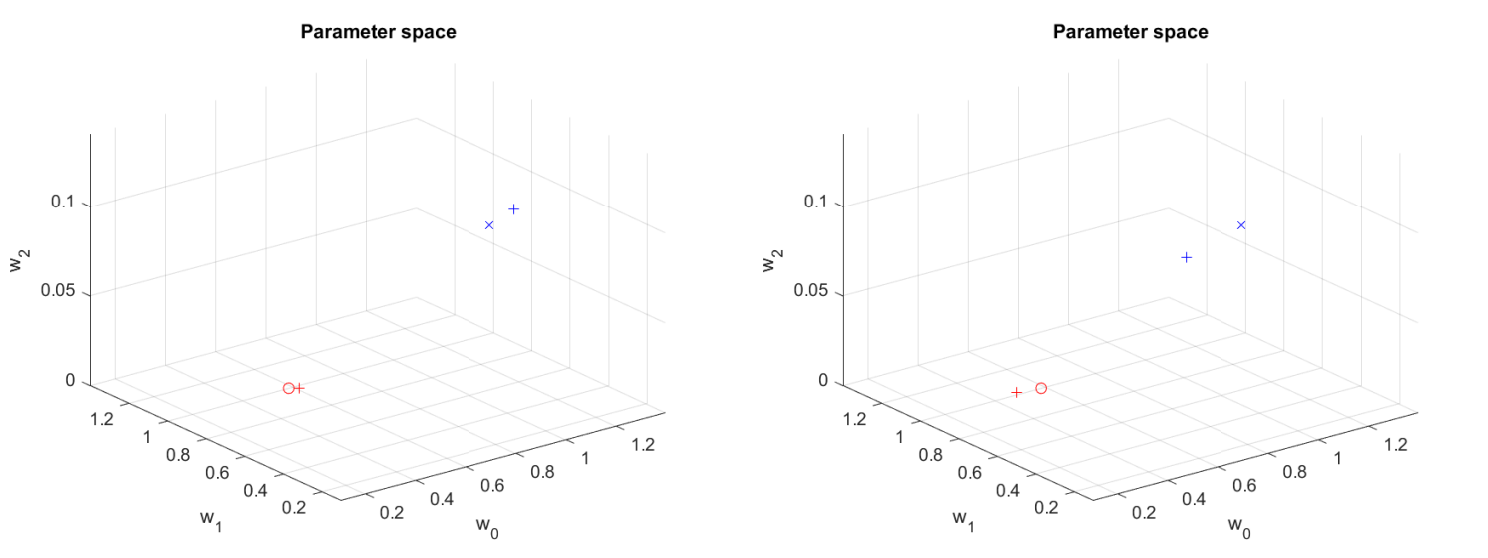
\includegraphics[width=0.75\linewidth]{images/bias1.png}
\end{figure}
In the Probabilistic Risk Minimization (PRM) framework, the blue $\times$ symbolizes the top-performing model within $\mathcal{H}_2$, while the red $\circ$ denotes the best model within $\mathcal{H}_1$.

For the Empirical Risk Minimization (ERM) perspective, the $+$ signifies the optimal parameters discovered for two instances of the dataset $\mathcal{D}$, each comprising $N = 1000$ samples.

If we conduct ERM iteratively across multiple trials, generating a hundred independent datasets, with varying sample sizes ($N = 100$ on the left and $N = 10000$ on the right).
\begin{figure}[H]
    \centering
    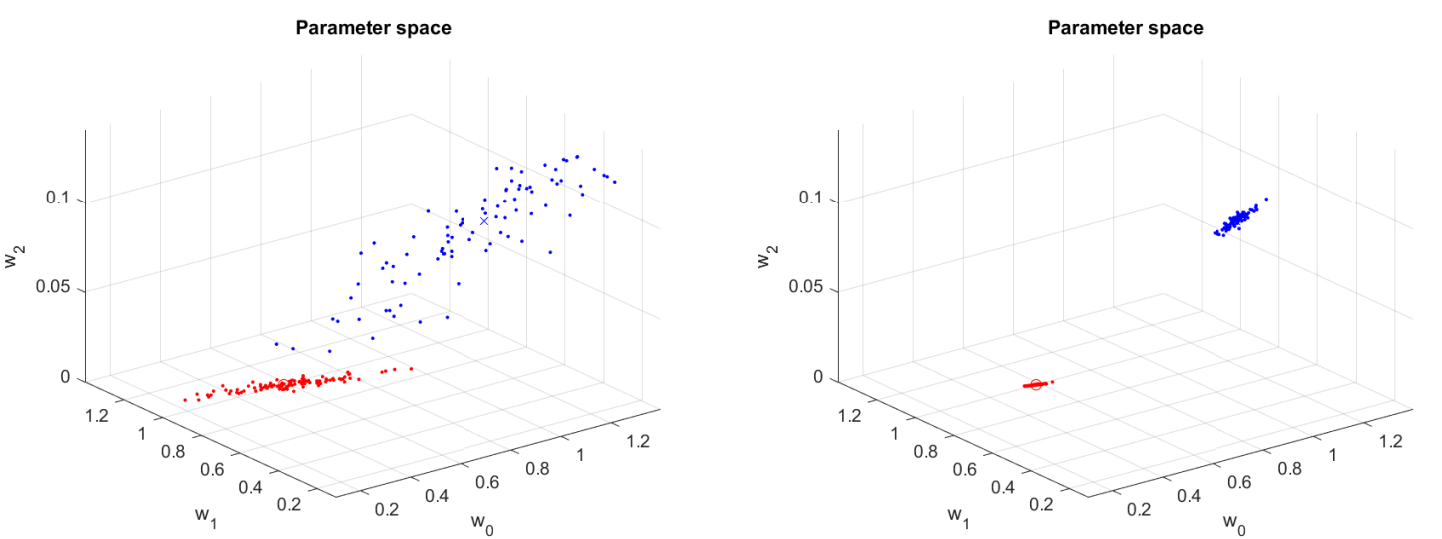
\includegraphics[width=0.75\linewidth]{images/bias2.png}
\end{figure}

\subsection{Error}
The error can be expressed as:
\[\mathbb{E}_{\mathcal{D},t}\left[{\left(t-\hat{y}(x)\right)}^2\right]=\sigma^2+\text{Var}_{\mathcal{D}}\left[\hat{y}(x)\right]+\mathbb{E}_{\mathcal{D}}{\left[f(x)-\hat{y}(x)\right]}^2\]
Here: 
\begin{itemize}
    \item $\mathbb{E}{\mathcal{D},t}\left[{\left(t-\hat{y}(x)\right)}^2\right]$ represents the expected error, computed with respect to the training dataset $\mathcal{D}$ and the target $t$.
    \item $\sigma^2$ denotes the irreducible error.
    \item $\text{Var}{\mathcal{D}}\left[\hat{y}(x)\right]$ stands for the variance, which diminishes with an increase in the number of samples $N=\left\lvert \mathcal{D}\right\rvert$.
    \item $\mathbb{E}_{\mathcal{D}}{\left[f(x)-\hat{y}(x)\right]}^2$ represents the bias, influenced by the hypothesis space $\mathcal{H}$.
\end{itemize}